\documentclass[10pt,a4paper]{article}
\usepackage[utf8]{inputenc} % para poder usar tildes en archivos UTF-8
\usepackage[spanish]{babel} % para que comandos como \today den el resultado en castellano
\usepackage{a4wide} % márgenes un poco más anchos que lo usual
\usepackage{caratula}
% \usepackage[left=3cm,right=3cm,bottom=3cm,top=3cm]{geometry}

% Comandos para formato
\usepackage[table,xcdraw]{xcolor}
\usepackage{hyperref}

% Comandos para simbolos matematicos.
\usepackage{amsmath, amssymb, tabularx}

% Comandos para referencias
\usepackage{natbib}

% Comandos para Figuras, Graficos, Tikz etc.
\usepackage{tikz}
\usepackage{epsfig}
%\usepackage{pgfplots}
\usepackage{graphicx}
\usepackage{epsfig}
\usepackage{caption}
\usepackage{subcaption}
\usepackage{svg}

% Comandos para teoremas etc.
\usepackage{amsthm}
\newtheorem{theorem}{Teorema}
\newtheorem{lemma}[theorem]{Lema}
\newtheorem{proposition}[theorem]{Proposición}
\newtheorem{remark}{Observación}
\newtheorem{corollary}{Corolario}
% \newproof{proof}{Demostración}

% Comandos para algoritmos.
\usepackage[noend]{algpseudocode}
\usepackage{algorithm}
\algnewcommand{\IfThenElse}[3]{% \IfThenElse{<if>}{<then>}{<else>}
\State \algorithmicif\ #1\ \algorithmicthen\ #2\ \algorithmicelse\ #3}
\algnewcommand{\IfThen}[2]{% \IfThenElse{<if>}{<then>}
  \State \algorithmicif\ #1\ \algorithmicthen\ #2}


\begin{document}

\titulo{TP 2: Problema del viajante de comercio}
\materia{Algoritmos y estructuras de datos III}

\integrante{La Ruffa, Franco}{404/19}{francolr97@gmail.com}
\integrante{Loria, Ezequiel}{111/16}{c03iif@hotmail.com}
\integrante{Asmad, Victor}{760/19}{vasmad@dc.uba.ar}
\integrante{Cesaroni, Mateo}{394/20}{mateocesaroni@gmail.com}

\maketitle

\section{Introducción} \label{sec:Intro}
El TSP (Travelling Salesman Problem) o Problema del Viajante de comercio en español, es un problema muy estudiado en el área de las ciencias de la computación
Esta incógnita consta de responder la siguiente pregunta:
Dada una lista de ciudades y la distancia entre cada par de ellas ¿Cual es la ruta mas corta posible que visita cada ciudad exactamente una vez y finaliza al regresar a la ciudad origen?
Esta respuesta trae consigo el denominado Camino Hamiltoniano, nombrado así en honor a W.R. Hamilton quien definió el problema en los años 1800s

A día de hoy, no se conocen algoritmos exactos que puedan devolver resultados en tiempos aceptables, es decir polinomiales, por lo cual se considera al mismo como un problema NP-Hard
Para la resolución del problema que se explicará a lo largo de todo este trabajo, se hará un recorrido por diversas técnicas denominadas Heurísticas cuyo objetivo es obtener diversos resultados aproximándonos mas a los óptimos globales, o en peor caso, los óptimos locales. Se define un óptimo local como un valor válido y de costo menor a otros y, el óptimo global como el mejor resultado entre todos los recorridos posibles

Dicho esto, comencemos

\section{Descripción del problema}
Un comerciante desea vender sus productos pasando por una cierta cantidad de destinos solo \textit{una vez} y tomando el camino \textit{más corto}.

Un viaje puede representarse por un grafo \textit{G=(V,E)} donde cada destino es un vértice y si existe un camino directo entre dos vértices distintos ese camino se denomina arista. El problema del viajante de comercio (de ahora en adelante TSP:\textit{Travelling Salesman Problem}) se resuelve si existe el camino más corto que visita todos los vértices una vez y permite que el viajante regrese a su posición inicial.

Los problemas de TSP pueden dividirse en dos tipos: aquellos problemas donde hay una arista entre todo par de vértices distintos, y aquellos donde no. En este trabajo práctico nos vamos a en focalizar solo en el primer tipo. 

\subsection{Ejemplo en la vida real}
Consideremos a un taxista que debe llevar cuatro personas a sus respectivas casas un sábado a la 08:00 a.m. luego de que las mismas salgan de un bar. Como el taxista sabe que hay muchas personas queriendo regresar a sus casas va a tratar de llevar la mayor cantidad que pueda, esto se logra iniciando en la puerta del bar, llevando a sus pasajeros y regresando al mismo lo más rápido posible para repetir el proceso; el taxista necesita, por lo tanto, tomar el camino más corto entre casa y casa para minimizar el tiempo de viaje y volver rápidamente al inicio para tomar más gente. En el grafo de abajo se puede ver una instancia del problema donde el taxista tiene que llevar a tres personas desde el bar \textit{vértice (1)} buscando la mínima distancia entre todas las casas de sus pasajeros y el inicio.

\begin{figure} [H]
    \centering
    \begin{subfigure}{0.4\linewidth}
        \centering
        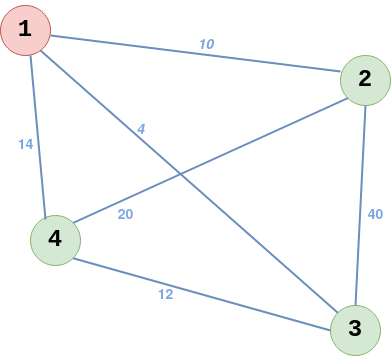
\includegraphics[scale=0.4]{img/taxi.png}
        \caption{El taxista: El coste óptimo es 46 recorriendo los nodos 1-2-4-3-1}
        \label{fig:camino taxista}
    \end{subfigure}
\end{figure}

\bigskip

\section{Descripción de los algoritmos}
En esta sección vamos a describir los algoritmos que se utilizaron para la resolución de este trabajo práctico. Los mismos son: Heurística constructiva golosa, Heurística basada en Árbol generador mínimo, Búsqueda local y Búsqueda Tabú

Para este algoritmo, las estructuras sobre las cuales se van a trabajar son grafos pesados completos, es decir, grafos densos. Este grafo no está orientado, esta decisión está tomada porque es indistinto ir desde $a$ hasta $b$ o viceversa puesto que solo voy a pasar por el nodo $a$ o $b$ una única vez por ejecución del algoritmo

Todos estos algoritmos reciben como input un grafo $G = (V, E)$ completo donde $\forall e \in E, e -> ei \forall i={1,...,n}$

Un detalle de implementación es que el grafo va a ser representado como una lista de adyacencias. Esto es un diccionario donde cada clave es el nodo y, cuyo significado, es una lista de tuplas. Cada tupla contiene dos datos importantes, uno es el vértice destino y el otro es el coste de la arista que une ambos objetivos

\subsection{Heurística constructiva golosa}

El primer algoritmo que se va a describir está basado en la aplicación de la Heurística Golosa Constructiva
Esta técnica se basa, aplicando un algoritmo goloso como se menciona en el nombre de la heurística, en empezar a partir de un nodo, llamémoslo $e_1$ y, a partir del mismo, ir recorriendo todo el grafo armando un camino simple.

La idea del algoritmo se basa en ir actualizando el ultimo nodo que estoy visitando, para esto llamemos $e_i con i={1,...,n}$ al i-ésimo nodo que estoy visitando tal que $e_{i-1} -> e_{i}$ puesto que se trata de un camino.
Para escoger un nuevo nodo, se miran todos los vecinos de $e_i$ y, entre todos aquellos se escoge el nodo cuya arista que une a $e_i$ con $e_{i+1}$ tenga menor peso
En todo momento, se tiene que estar revisando cuales vértices ya están incluidos en el camino con la finalidad de no volver de un nodo hacia otro que ya se haya visitado y, de esta forma, estar armando un ciclo intermedio

Una vez haya recorrido todos los nodos y, tenga un camino simple sin ciclos (dato importante puesto que se trata de un camino euclidiano y no pueden haber ciclos intermedios como se menciono al principio), entonces conecto el último nodo que haya recorrido, llamémoslo $e_n$, y uno $e_n$ con $e_1$ sea cual sea el peso de la arista
Se conecta el ultimo nodo con el primero puesto que, como se mencionó antes, el objetivo de este problema es armar un camino que inicie y termine en el mismo nodo desde el que partí y que, a su vez, no hayan ciclos intermedios

En la aplicación hecha del algoritmo, existe una constante la cual va conservando la suma de las aristas hasta el momento
El algoritmo termina cuando haya encontrado un camino euclidiano, esto es, cuando en el camino estén todos los nodos del grafo original y, una vez suceda esto, se une el ultimo nodo del mismo con el primero. Si esto es posible, devuelve un camino con su coste, caso contrario, se informa que no hay un camino posible

\begin{algorithm}[H] 
\caption{Algoritmo de Búsqueda Golosa Constructiva}
\begin{algorithmic}[1]
\State costoFinal $\gets$ 0
\Function{$BG$}{$Grafo G$}
    \State S $\gets$ []
    \State Vértice n $\gets$ algún vértice cualquiera de V(G)
    \State costoAux $\gets \infty$
    \State para cada $e \in d(v)$
    \If{e(v) $\not\in S$}
        costoFinal $\gets$ costoFinal + $c_i$
    \EndIf
    costoFinal $\gets$ costoFinal + $(e_n \rightarrow e_i)$
\EndFunction
\end{algorithmic}
\label{alg:bg}
\end{algorithm}

El algoritmo mencionado devuelve un camino euclidiano en el cual, se encuentran todos los nodos del grafo
Con esto en cuenta, la complejidad del algoritmo se mide en base a los recorridos de los nodos ya que, en cada paso estoy tomando una aristas que une al nodo $e_i$ con el nodo $e_j$ vecino. Es decir, en cada iteración, estoy recorriendo todos los vecinos del nodo $e_i$ y tomando el que tenga arista de menor costo. Esto se realiza en $O(d(e_i))$

A su vez, recorro todos los nodos a lo sumo una vez, esto es $O(V)$ y también todos los vértices puesto que si estoy mirando todos los vecinos de cada nodo, a lo sumo reviso dos veces cada arista. Esto es porque ocurre en varios casos que miro el coste de la arista $e_i -> e_j$ y $e_j -> e_i$ pero en alguno de los dos casos, uno de los nodos ya está agregado al camino, entonces veo dos veces cada arista. Esto resulta en $O(E)$

Luego la complejidad es $O(V) + O(E) + O(d(e_i)) > O(V) + O(E)$ y, como se trata de un grafo completo, es un grafo denso, por lo tanto tengo a lo sumo $O(V^2)$ aristas. Finalmente, la complejidad del algoritmo es $O(V^2)$

No tenemos que olvidarnos tampoco de la complejidad espacial. Como buscamos un camino euclidiano, nos basta con tener una estructura de lista con tamaño $|V|$ puesto que lo que voy a tener son, en orden, todos los vértices que se visitan
Si quiero las aristas individuales, me basta revisar en el grafo, la arista de la lista en posición $ij$ y obtengo el peso de la arista. Por lo tanto, como complejidad espacial se obtiene $O(V)$

\subsection{Heurística basada en AGM}

El segundo algoritmo está basado en la técnica de Heurística Basada en Árbol Generador Mínimo. La misma consta en utilizar un árbol generador mínimo como dice el nombre de la heurística y, posteriormente, utilizar otro algoritmo para recorrer el mismo obteniendo en este ultimo caso, el orden de visita a cada vértice del AGM
Obtenido el orden de visita, se obtienen las aristas que cumplen que el resultado final sea un camino euclidiano y se cierra el ciclo, obteniendo de esta forma un camino válido

Respecto a la resolución de este algoritmo, se optó por utilizar para obtener el AGM, el algoritmo de Prim ya que, en cada iteración va generando un árbol que va cumpliendo con lo pedido, a demás, se nos hizo mas fácil la implementación del mismo
Y, para recorrer árbol, se escogió DFS (Depth First Search) ya que este algoritmo recorre todo el grafo brindando información sobre la estructura del mismo y, obteniendo de esta forma, un orden para recorrer el resultado final

Tanto Prim como DFS son algoritmos golosos. Estos algoritmos van, en cada iteración, escogiendo la arista que tenga menor peso, siendo en parte similar a la Heurística Golosa Constructiva. No obstante, la aplicación de DFS para obtener el orden diferencia al mismo puesto que puede traernos mejores resultados al final, resultados con aristas que no tengan un peso exorbitante. Este tema se tratará posteriormente en la parte de experimentación
 
 Los pasos para la resolución de este algoritmo son los siguientes:
 \begin{itemize}
     \item Se obtiene un AGM a partir del grafo original
     \item Se aplica DFS sobre el AGM
     \item Se recorre el orden de los nodos
     \item Obtenido un camino simple, se cierra el ciclo y se devuelve el camino junto con su costo
 \end{itemize}

\begin{algorithm}[H]
\caption{Algoritmo de Heurística en Árbol Generador Mínimo}
\begin{algorithmic}[1]
\State costoFinal $\gets$ 0
\Function{$AGM$}{$Grafo G$}
    \State Grafo S $\gets$ []
    \State Grafo G' $\gets$ BG(g)
    \State Grafo G'' $\gets$ DFS(G')
    \State para cada $e_i \in G'$
        \State costoFinal $\gets costoFinal + e_i$
\EndFunction
\end{algorithmic}
\label{alg:AGM}
\end{algorithm}

La complejidad de este algoritmo se basa principalmente en la complejidad del algoritmo escogido para obtener el árbol generador mínimo
Al tratarse de un grafo denso, el costo de ejecución de este algoritmo puede llegar a $O(|V|^2)$ ya que se tienen que recorrer a lo sumo $|V|^2$ aristas
El algoritmo DFS se recorre sobre el AGM, entonces la complejidad del mismo es lineal respecto al resultado del algoritmo previo
Unir la ultima arista con la primera se realiza en O(1) dependiendo de la estructura utilizada

Si se considera algún que otro cambio en la ejecución del algoritmo, este puede extenderse un poco en tiempo, es decir, ir buscando los vecinos de un nodo que esté visitado dos veces por como esta armado el AGM y hacer este cambio. Teniendo esto en cuenta, podemos saber que el algoritmo no tendrá mas de 2 veces el coste del AGM. Finalmente, la complejidad es $O(|V|^2)$

\subsection{Búsqueda local}
El tercer algoritmo se basa en la técnica de búsqueda local Esta es una heurística enfocada en la optimización de problemas difíciles. 

El objetivo de esta heurística es, dada alguna solución valida, buscar otras soluciones con mejores resultados aplicando cambios locales hasta que se encuentre un resultado óptimo o pase un limite de tiempo.

Para la resolución de este problema, consideramos esta solución válida estará basada en un camino hamiltoniano $S$ y el costo de recorrerlo $c$, entonces la forma de obtener otros valores consta de buscar los vecinos de $S$. A este conjunto, se lo denomina la vecindad.

Para ello, definimos la vecindad como $Vecindad(S) = (S' | S' = swap(S, i, j) para i, j en (1,...,n))$. Esto se obtiene de aplicar la técnica  2-opt que consiste en, dados 4 vértices en la solución original, intercambiar las aristas que las unen. Esto lo podemos hacer puesto que G es un grafo completo, si no, no sería válido. Entonces, sean $a, b, c, d \in E$, $a->b$ y $c->d$ vértices unidos por sus aristas en el camino $S$, el resultado obtenido después de intercambiar aristas es $a->c$ y $d->b$. Este cambio nos permite obtener otro camino válido que se denomina vecino de $S$ ya que surge a partir de usarlo para generar otro. Entonces, definimos la vecindad como: $Vecindad(S) = (S' | S' = swap(S, i, j) para i, j en (1,...,n))$

Dijimos previamente que para realizar una búsqueda local, se necesita un camino válido ya calculado. Para esto se decidió tomar el camino generado por la heurística {heurística} puesto que, luego de varias pruebas que se explicarán mas adelante en la sección de experimentación, nos devuelve un camino válido con un coste mucho menor que la heurística {heurística}. Entonces, teniendo ya un camino con un coste aceptable, buscamos la vecindad del mismo para buscar una mejor solución.

El algoritmo finaliza cuando no puede encontrar una solución mejor a la ultima ya encontrada
Luego, el algoritmo se define como:

\begin{algorithm}[H] 
\caption{Algoritmo de Búsqueda Local}
\begin{algorithmic}[1]
\State costoFinal $\gets$ 0
\Function{Búsqueda Local}{$Grafo G$}
    \State S $\gets$ BG(G)
    \State hayMejora $\gets$ true
    \State solOptima $\gets$ S
    \While{hayMejora} \label{lst:line:blwhile}
        \State Vec $\gets$ Vecindad(S)
        \If{costo(Vec) $<$ costo(S)}
            S $\gets$ Vec
        \EndIf
        \If{costo(Vec) $>$ costo(S)}
            hayMejora $\gets$ false
        \EndIf
    \EndWhile
\EndFunction
\end{algorithmic}
\label{alg:BL}
\end{algorithm}

Debido a que el algoritmo se detiene cuando no encuentra una mejora al ver los vecinos, definimos una variable cantDeMejoras que va a representar la cantidad de iteraciones en donde encontró una mejor solución (linea \ref{lst:line:blwhile}) para poder explicar correctamente la complejidad. \\
Obtener el vecindario tiene costo $O(n^2)$ ya que para cada vértice, hago permutaciones con los demás vértices
El obtener el costo del camino implica recorrer una lista de tamaño N ($O(N)$) revisando las aristas de vec[i],vec[i+1] también en $O(N)$ ya que las ve mediante lista de adyacencia en donde ubica al vértice i en $O(1)$ y recorre sus vecinos en $O(N)$. Finalmente la complejidad es $O(N^2)$ \\
Con todo esto en cuenta, hacemos se hace el calculo de la complejidad:
$O(AGM) + (O(N^2) + O(N^2)) * O(cantDeMejoras) = O(AGM) + 2O(N^2)*O(cantDeMejoras) \equiv O(cantDeMejoras*O(n^2)$ 
Finalmente, resumimos que la complejidad de obtener una solución válida resulta en $O(cantDeMejoras*O(n^2)$ 

\subsection{Heurística de Búsqueda Tabú}
El ultimo algoritmo que vamos a utilizar está basado en la meta heurística de la Búsqueda tabú. Este método surge como una aplicación de la búsqueda local (ya presentada en el algoritmo anterior) para obtener mejores resultados

La razón de este uso es, que mientras la búsqueda local puede quedarse en óptimos locales buscando en cierta vecindad de la solución y, siempre avanza buscando una mejor solución, la búsqueda tabú se puede permitir el tomar resultados peores con la finalidad de, en una próxima iteración buscando otra solución, obtengamos un resultado mucho mejor que sin haber tomado esta decisión

En algunos casos, el realizar esta acción de permitirse ir por peores resultados para luego encontrar uno mejor, permite que se pueda encontrar un óptimo global frente a un óptimo local como si sucedería con la búsqueda local

Para poder obtener mejores soluciones, nos basamos en la búsqueda local, especialmente vamos a enfocarnos en la técnica 2-opt para la cual, daremos ciertos parámetros que nos permitan extender los resultados y obtener mejores valores, estos se denominan, los componentes los cuales nos dan control sobre el mismo 

Como componentes nos vamos a enfocar en los siguientes items:
\begin{itemize}
    \item Criterios de parada - Cantidad de iteraciones: Este parámetro limita la cantidad de operaciones o, iteraciones, que se pueden realizar para obtener mejores resultados. Por iteración nos referimos a la cantidad de vecindades que podemos obtener dado el ultimo resultado obtenido, de esta forma limitamos cuanto podemos buscar dentro del vecindario de la solución ya que, puede ocurrir que la cantidad de vecinos sea incluso infinita si tenemos infinitos vértices, si no limitamos este parámetro, podemos quedarnos iterando eternamente
    
    \item Subconjunto de vecindad - 2opt + Random : Este parámetro consiste en, dada una solución $S$ y $Vecindad(S)$, de todos los posibles valores en la vecindad, tomamos un porcentaje random de los resultados, es decir, los caminos con aristas cambiadas
    
    \item Memoria : Para este item, se decidió utilizar una lista como estructura de memoización
    \begin{itemize}
        \item Recordar Ciclos : En cada iteración se recuerda el camino entero obtenido sobre el cual, posteriormente, se buscarán mejores resultados
        \item Recordar Swaps : Dado un camino S' resultado de aplicar la operación swap, se recordarán los vértices que intercambiaron de aristas para formar una nueva vecindad
    \end{itemize}
    En el algoritmo utilizado se aplicarán ambos tipos de memoria, por ende tenemos un parámetro que nos indicará que tipo de memoria utilizar y, dependiendo del mismo, podemos obtener incluso distintos resultados
    El porque de usar la memoria consiste en, que si un ciclo o un swap ya ha sido visitado, no se vuelva a visitar en alguna próxima iteración donde haya algo similar
    Por ejemplo: Es lo mismo el camino que contenga a la arista $a\rightarrow b$ como $b \rightarrow a$ pues el grafo no es dirigido
    La misma idea ocurre con memorizar los ciclos
    
    \item Aspiración
    Este ultimo componente consiste en recordar en todo momento la mejor solución vista hasta el momento. Esta será considerado nuestro resultado final hasta que encontremos uno mejor, en tal caso, hacemos el cambio
    
\end{itemize}

Como solución inicial elegimos el camino obtenido por el algoritmo {alg}
Teniendo esto en cuenta, definimos el pseudocódigo del algoritmo como:

\begin{algorithm}[H]
\caption{Algoritmo de Búsqueda Tabú}
\begin{algorithmic}[1]
\State costoFinal $\gets$ 0
\Function{Búsqueda Tabú}{$G: Grafo$}
    \State S $\gets$ AGM(G)
    \State sol $\gets$ S
    \State iteración $\gets$ 0
    \While{mientras iteración $<$ $iteracionesMax$} \label{lst:line:tabuiteracion}
        \State subVec $\gets$ obtenerSubVecindad(S, porcentaje)   \label{lst:line:tabuvecindad}
        \State mejorEnSubVec $\gets$ obtengo el mejor en la subvecindad de S    \label{lst:line:tabumejor}
        \If{coste(sol) < coste(S)} 
            \State S $\gets$ sol   \label{lst:line:tabuaspiracion}
        \EndIf
    \EndWhile
\EndFunction
\end{algorithmic}
\label{alg:TABU}
\end{algorithm}

\begin{algorithm}[H]
\caption{Algoritmo de obtención de SubVecindad}
\begin{algorithmic}[1]
\Function{obtenerSubVecindad}{$G: Grafo$, $porcentaje: \mathbb{R}$}
    \State vecinos $\gets$ []
    \State i, j $\gets$ 0
    \While{i $\leq$ n}
        \While{j $\leq n$}
            \State vecinos $\gets Ag(vecinos, swap(G, i, j))$
            \State j $\gets$ j + 1
        \EndWhile
        \State i $\gets$ i + 1
    \EndWhile
    \State SubVecindad $\gets$ []
    \While{$|vecindario| < vecinos*porcentaje$}
        \State $Ag(vecindario, dameUno(vecinos)$
    \EndWhile
    \State devolver SubVecindad
\EndFunction
\end{algorithmic}
\end{algorithm}

\begin{algorithm}[H]
\caption{Algoritmo de mejorSubvecino}
\begin{algorithmic}[1]
\Function{mejorSubvecino}{$Grafo G, subVecindad sv , memoria memo$}
    \State mejor $\gets$ INFTY
    \State mejorOrden $\gets$ 0
    \State swap $\gets$ []
    \State mejorSwap $\gets$ []
    \If{tipoMemo$==Ciclo$}
        \State i $\gets$ 0
        \While{$i<len(sv)$}
            \If{sv[i] $\notin$ memo}
                sol $\gets$ costo(sv[i])
                \If{sol$<$mejor}
                    \State mejor $\gets$ sol
                    \State mejorOrden $\gets$ sv[i]
                \EndIf
            \EndIf
        \EndWhile
        \If{len(memo)$<$tamanioMemo}
            \State $Ag(memo,sv[i])$
        \EndIf
        \If{len(memo)$==$tamanioMemo}
            \State $memo.pop_front()$
            \State $Ag(memo,sv[i])$
        \EndIf
    \EndIf
    \If{tipoMemo$==$swap}
        \State i $\gets$ 0
        \While{$i<len(sv)$}
            \State swap $\gets$ swapEn(sv[i]) 
            \If{swap $\notin$ memo}
                sol$\gets$ costo(sv[i])
                \If{sol<mejor}
                    \State mejor $\gets$ sol
                    \State mejorOrden $\gets$ sv[i]
                    \State mejorSwap $\gets$ swap
                \EndIf
            \EndIf
         \EndWhile 
         \If{len(memo)$<$tamanioMemo}
            \State $Ag(memo,swap)$
        \EndIf
        \If{len(memo)$==$tamanioMemo}
            \State $memo.pop_front()$
            \State $Ag(memo,swap)$
        \EndIf
    \EndIf
\State mejorSv $\gets (mejor,mejorOrden)$
\State devolver mejorSv
\EndFunction
\end{algorithmic}
\end{algorithm}

%complejidad sol inicial + (subvec= max(n^2,filtrar) + obtenermejor=(N^2*(tamañoMemo*N) + N))*CantIt = (max(n^2,filtrar)+tamañoMemo*N^3)*CantIt

El cálculo de complejidad de este algoritmo es distinto en relación a la búsqueda local pese a estar basado en el mismo y sus métodos. Para esto, analizaremos el algoritmo respecto a los valores de las componentes, esto es, Criterios de parada, Conjunto de subvecindad, memoria y Aspiración

Empecemos por Aspiración. Esta parte indica que se almacena siempre la mejor solución obtenida hasta el momento. Esto es un camino de $|V|$ vértices en memoria. O(n)

El algoritmo de obtención de la sub vecindad (linea \label{lst:line:tabuvecindad} consiste en, para todos los vértices obtener todas las permutaciones de este mismo e ir almacenándolos en una lista. El obtener todos estos vecinos tiene costo $O(n^2)$ ya que consiste en recorrer dos veces todos los vértices para permutar las aristas
Posteriormente, entra en juego el parámetro del conjunto de sub vecindad. Como este valor es un número que nos dice que porcentaje de todos los vecinos de la solución se toma, el peor caso consiste que el valor sea de 100 ya que ese valor representa el 100 de los vecinos, en tal caso, se llena una lista a devolver con todos los vecinos. Esto se hace puesto que, si el valor es inferior a 100, vamos tomando de manera aleatoria los vecinos y los colocamos en esta lista.
Para verificar si el vecino no fue agregado ya, usamos otra estructura de memoización de tamaño $|vecinos|$ donde tenemos O si no fue agregado y 1 si lo fue, esta estructura tiene tamaño $O(|vecinos|)$ como la que va a devolverse como respuesta.
Como para seleccionar que valores tomamos usamos una generación aleatoria, puede no ser uniforme la selección de que valore se toman y, para casos como un porcentaje de 50, puede pasar muchas veces por un mismo valor antes de cambiar a otro
Entonces la complejidad para este algoritmo consta de $O(max(n^2, filtro)$.

Luego tenemos el método para obtener el mejor de los vecinos. Para este método tenemos que tener en cuenta algo importante. Se reciben como parámetro el tipo de la memoria y el tamaño de la memoria.
Dependiendo del tipo de memoria la complejidad puede cambiar. Esto se debe a que, en la estructura de memoización se almacenan 2 tipos de datos, o ciclo o swap y, en cada iteración se busca si el valor se ha visitado antes o no. Dicha comparación se realiza a motivo de no repetir procesos innecesarios ya que recorrer una arista $(a,b)$ es lo mismo que recorrer $(b,a)$ por ejemplo. El costo de hacer una comparación del swap es O(1) puesto que se comparan tuplas de 2 valores
En el caso de los ciclos, puede ocurrir que para dos caminos distintos, un swap haga que los caminos queden iguales. En este caso, el costo de comparar se eleva a $|V|$ ya que, en la estructura, se guardan caminos enteros
Sumado a esto, en cada comparación se debe recorrer la estructura de memoización ya que es una lista que se va extendiendo mientras la memoria no se haya completado
Entonces, buscar si un valor está o no en la estructura tiene costo $O(tamanioMemoria*N)$.

Luego, hacemos esto por cada elemento en los vecinos. Por ende la complejidad incrementa a $O(cantVecinos*tamanioMemoria*N)$.
La cantidad de vecinos es a lo sumo $O(n^2)$ porque se permuta a lo sumo 2 aristas de cada camino, entonces el tiempo es acotado. Con esto, la complejidad es $O(n^3 * tamanioMemoria)$.

Finalmente, teniendo estos dos algoritmos, la complejidad es de $O(max(n^2, filtro)) + O(N^3*tamanioMemoria)$.
Esta complejidad se realiza cantIteraciones, que es el componente del criterio de parada.
Con esto en cuenta, la complejidad final del algoritmo asciende a: $O((max(n^2,filtrar)+tamanioMemo*N^3)*CantIt)$

\section{Experimentación}

\subsection{experimentos con datasets dados}
Para estos experimentos vamos a utilizar las siguientes instancias:
\begin{itemize}
\setlength{\itemsep}{1pt}
\setlength{\parskip}{0pt}
 \setlength{\parsep}{0pt}

\item \textbf{ulysses16}   
\item \textbf{berlin52}
\item \textbf{st70}
\item \textbf{kroE100}

\end{itemize}

Estas instancias fueron elegidas para las experimentaciones de Tabú ya que representan una variedad suficiente de tamaños de entrada y se consideró que ver otras instancias con N muy grande sería demasiado costoso con respecto al tiempo y sus resultados no serían lo suficientemente distintos a las instancias propuestas como para que sea de interés analizarlos. 

Para empezar, vamos a comparar los resultados de AGM y BG en las instancias presentadas anteriormente con la finalidad de decidir cual de los algoritmos se va a utilizar como solución inicial para búsqueda local y tabú.
% la idea seria empezar con una comparación entre BG y AGM así justificamos porque elegimos BG como sol inicial para Tabu.

\begin{figure} [H]
    \centering
    %\begin{subfigure}{0.5\linewidth}
    %\centering
    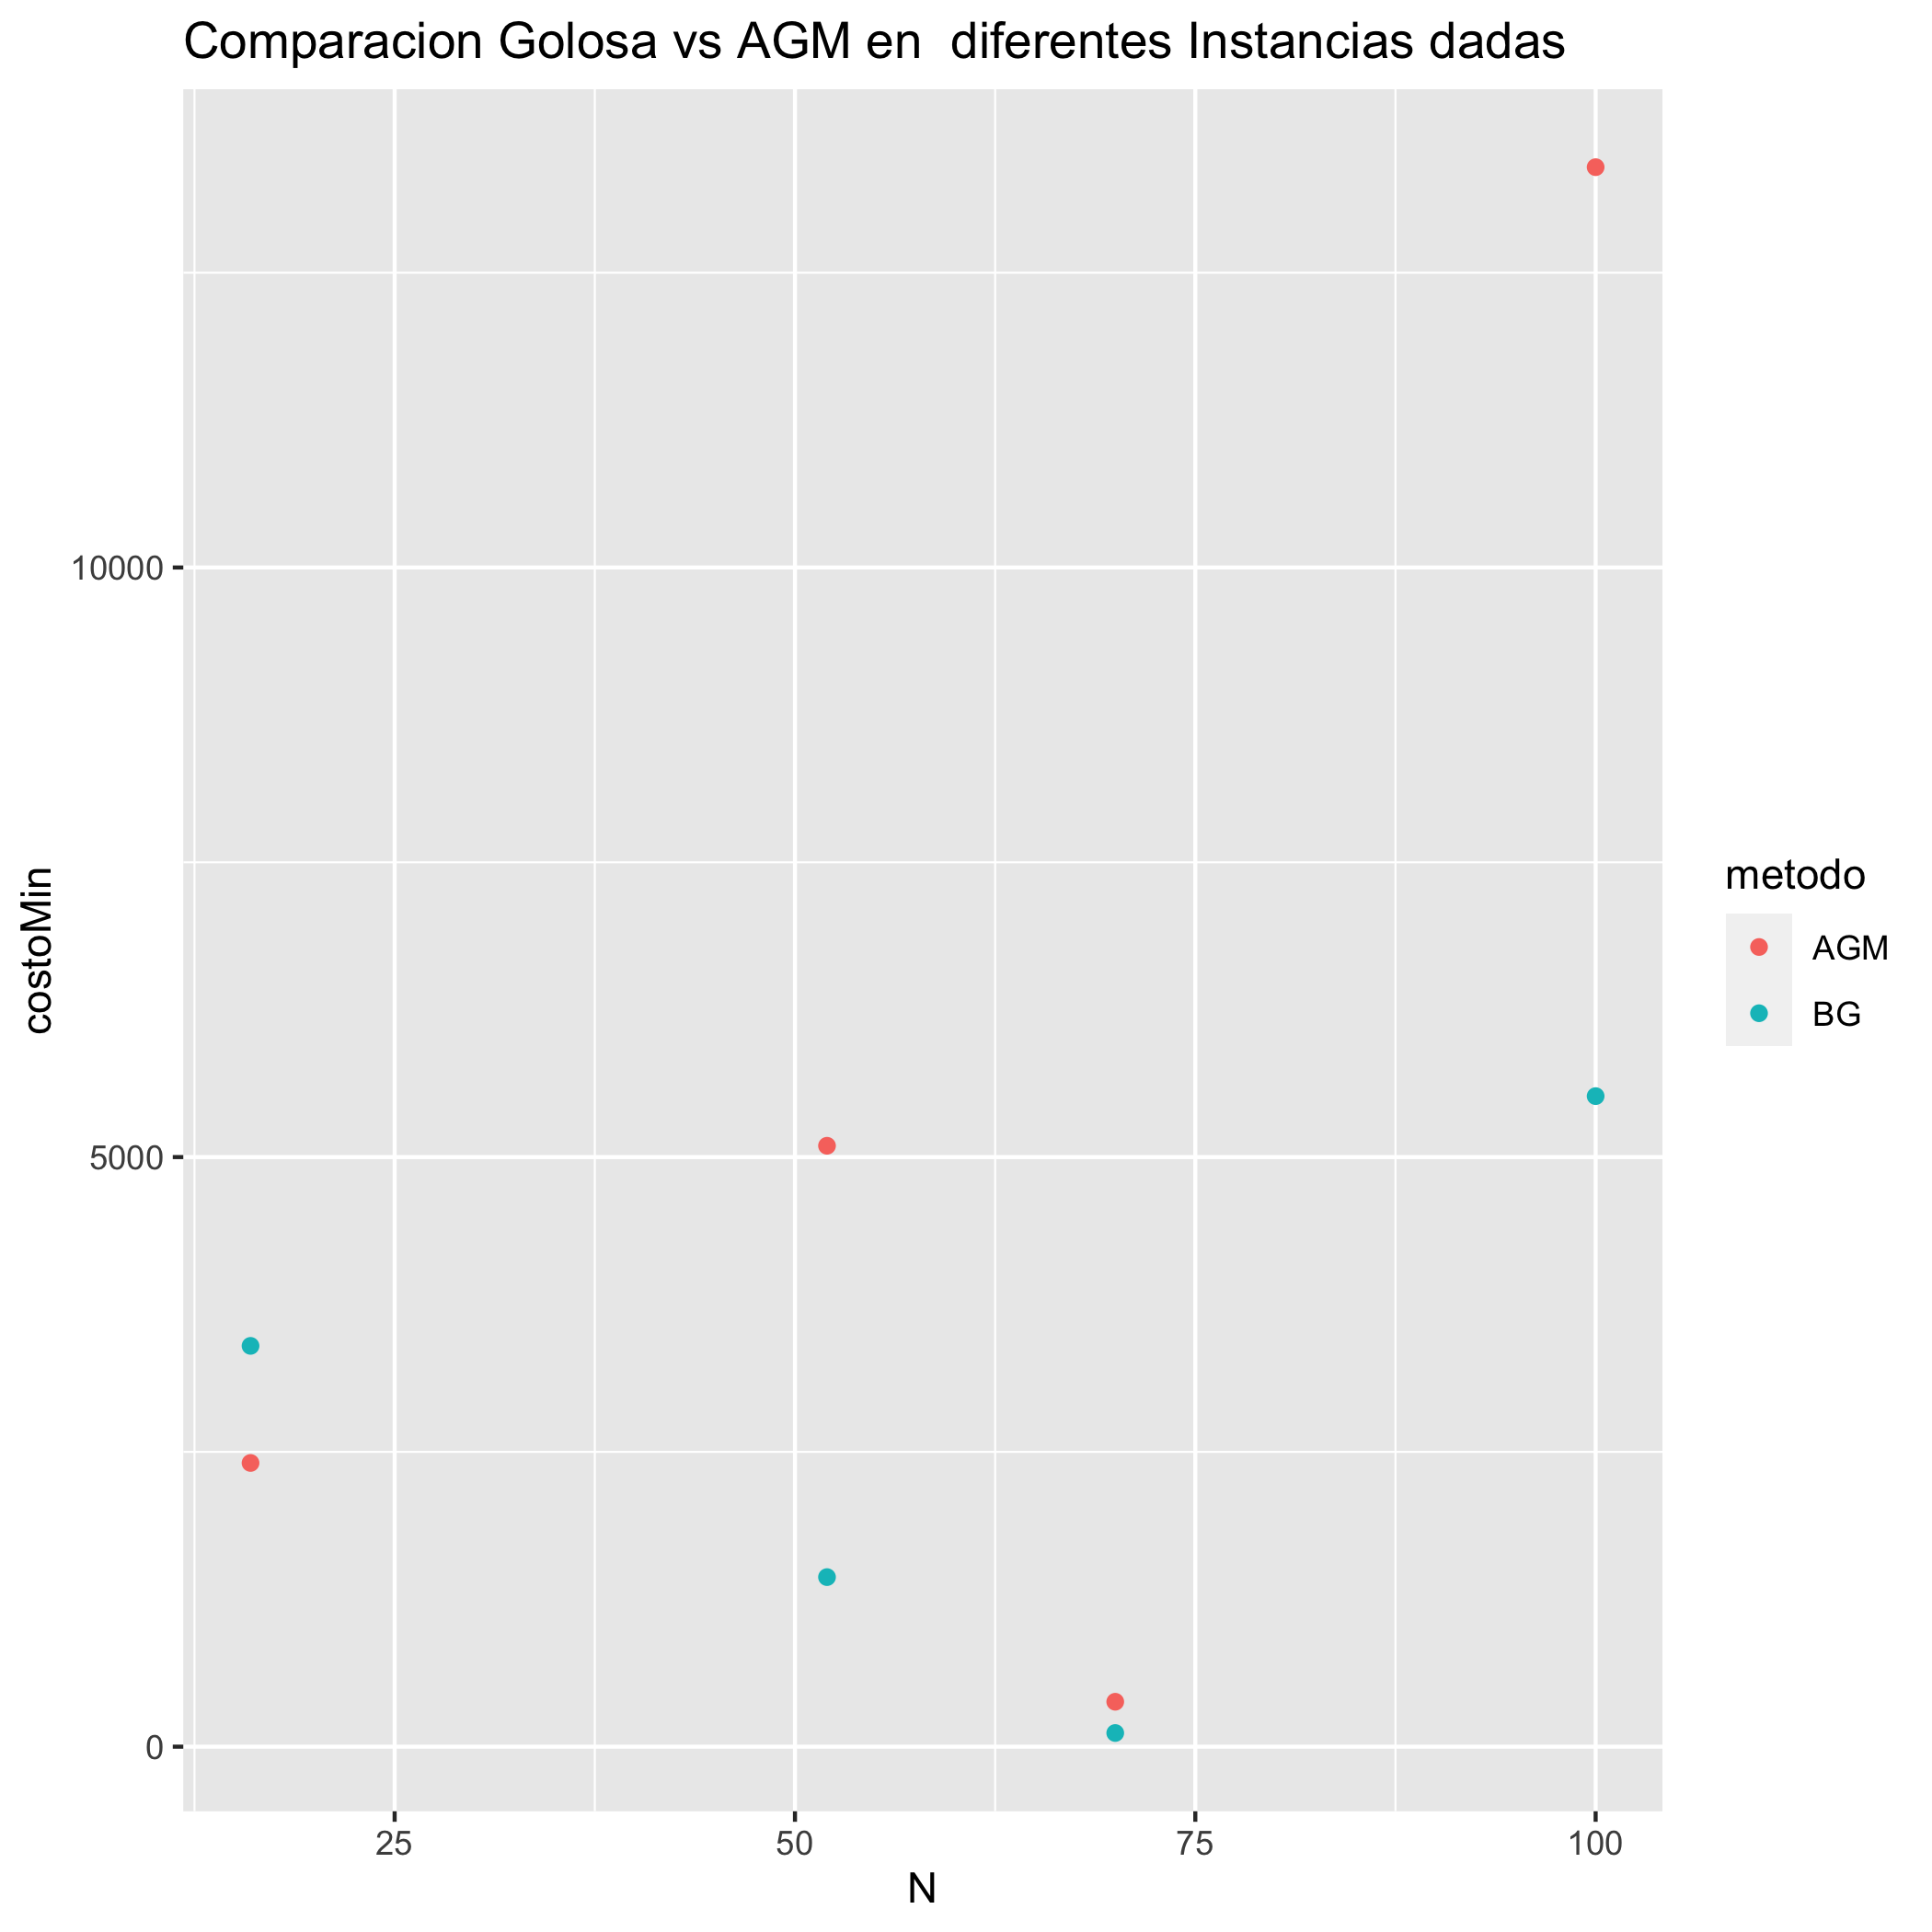
\includegraphics[scale=0.15]{img/AGMvsGolosa.png}
    \caption{comparación Agm vs BG}
    %\end{subfigure}
    \label{fig:agmvsbg}
\end{figure}

Como podemos observar en ~\ref{fig:agmvsbg}, en la mayoría de los casos probados la heurística golosa que implementamos en el algoritmo \ref{alg:bg} devuelve un costo más cercano al óptimo, por lo tanto vamos procedemos a utilizarla. \\

%Despues las comparaciones de los distintos parámetros y ver que va dando mejor y llegar a una conclusión de que combinación parecería ser la mas optima de usar.
Ahora vamos a analizar que tipos de parámetros son mejores para la resolución de Tabú: \\

Primero vamos a comparar el porcentaje de subvecindad: 

\begin{figure} [H]
    \centering
    %\begin{subfigure}{0.5\linewidth}
    %\centering
    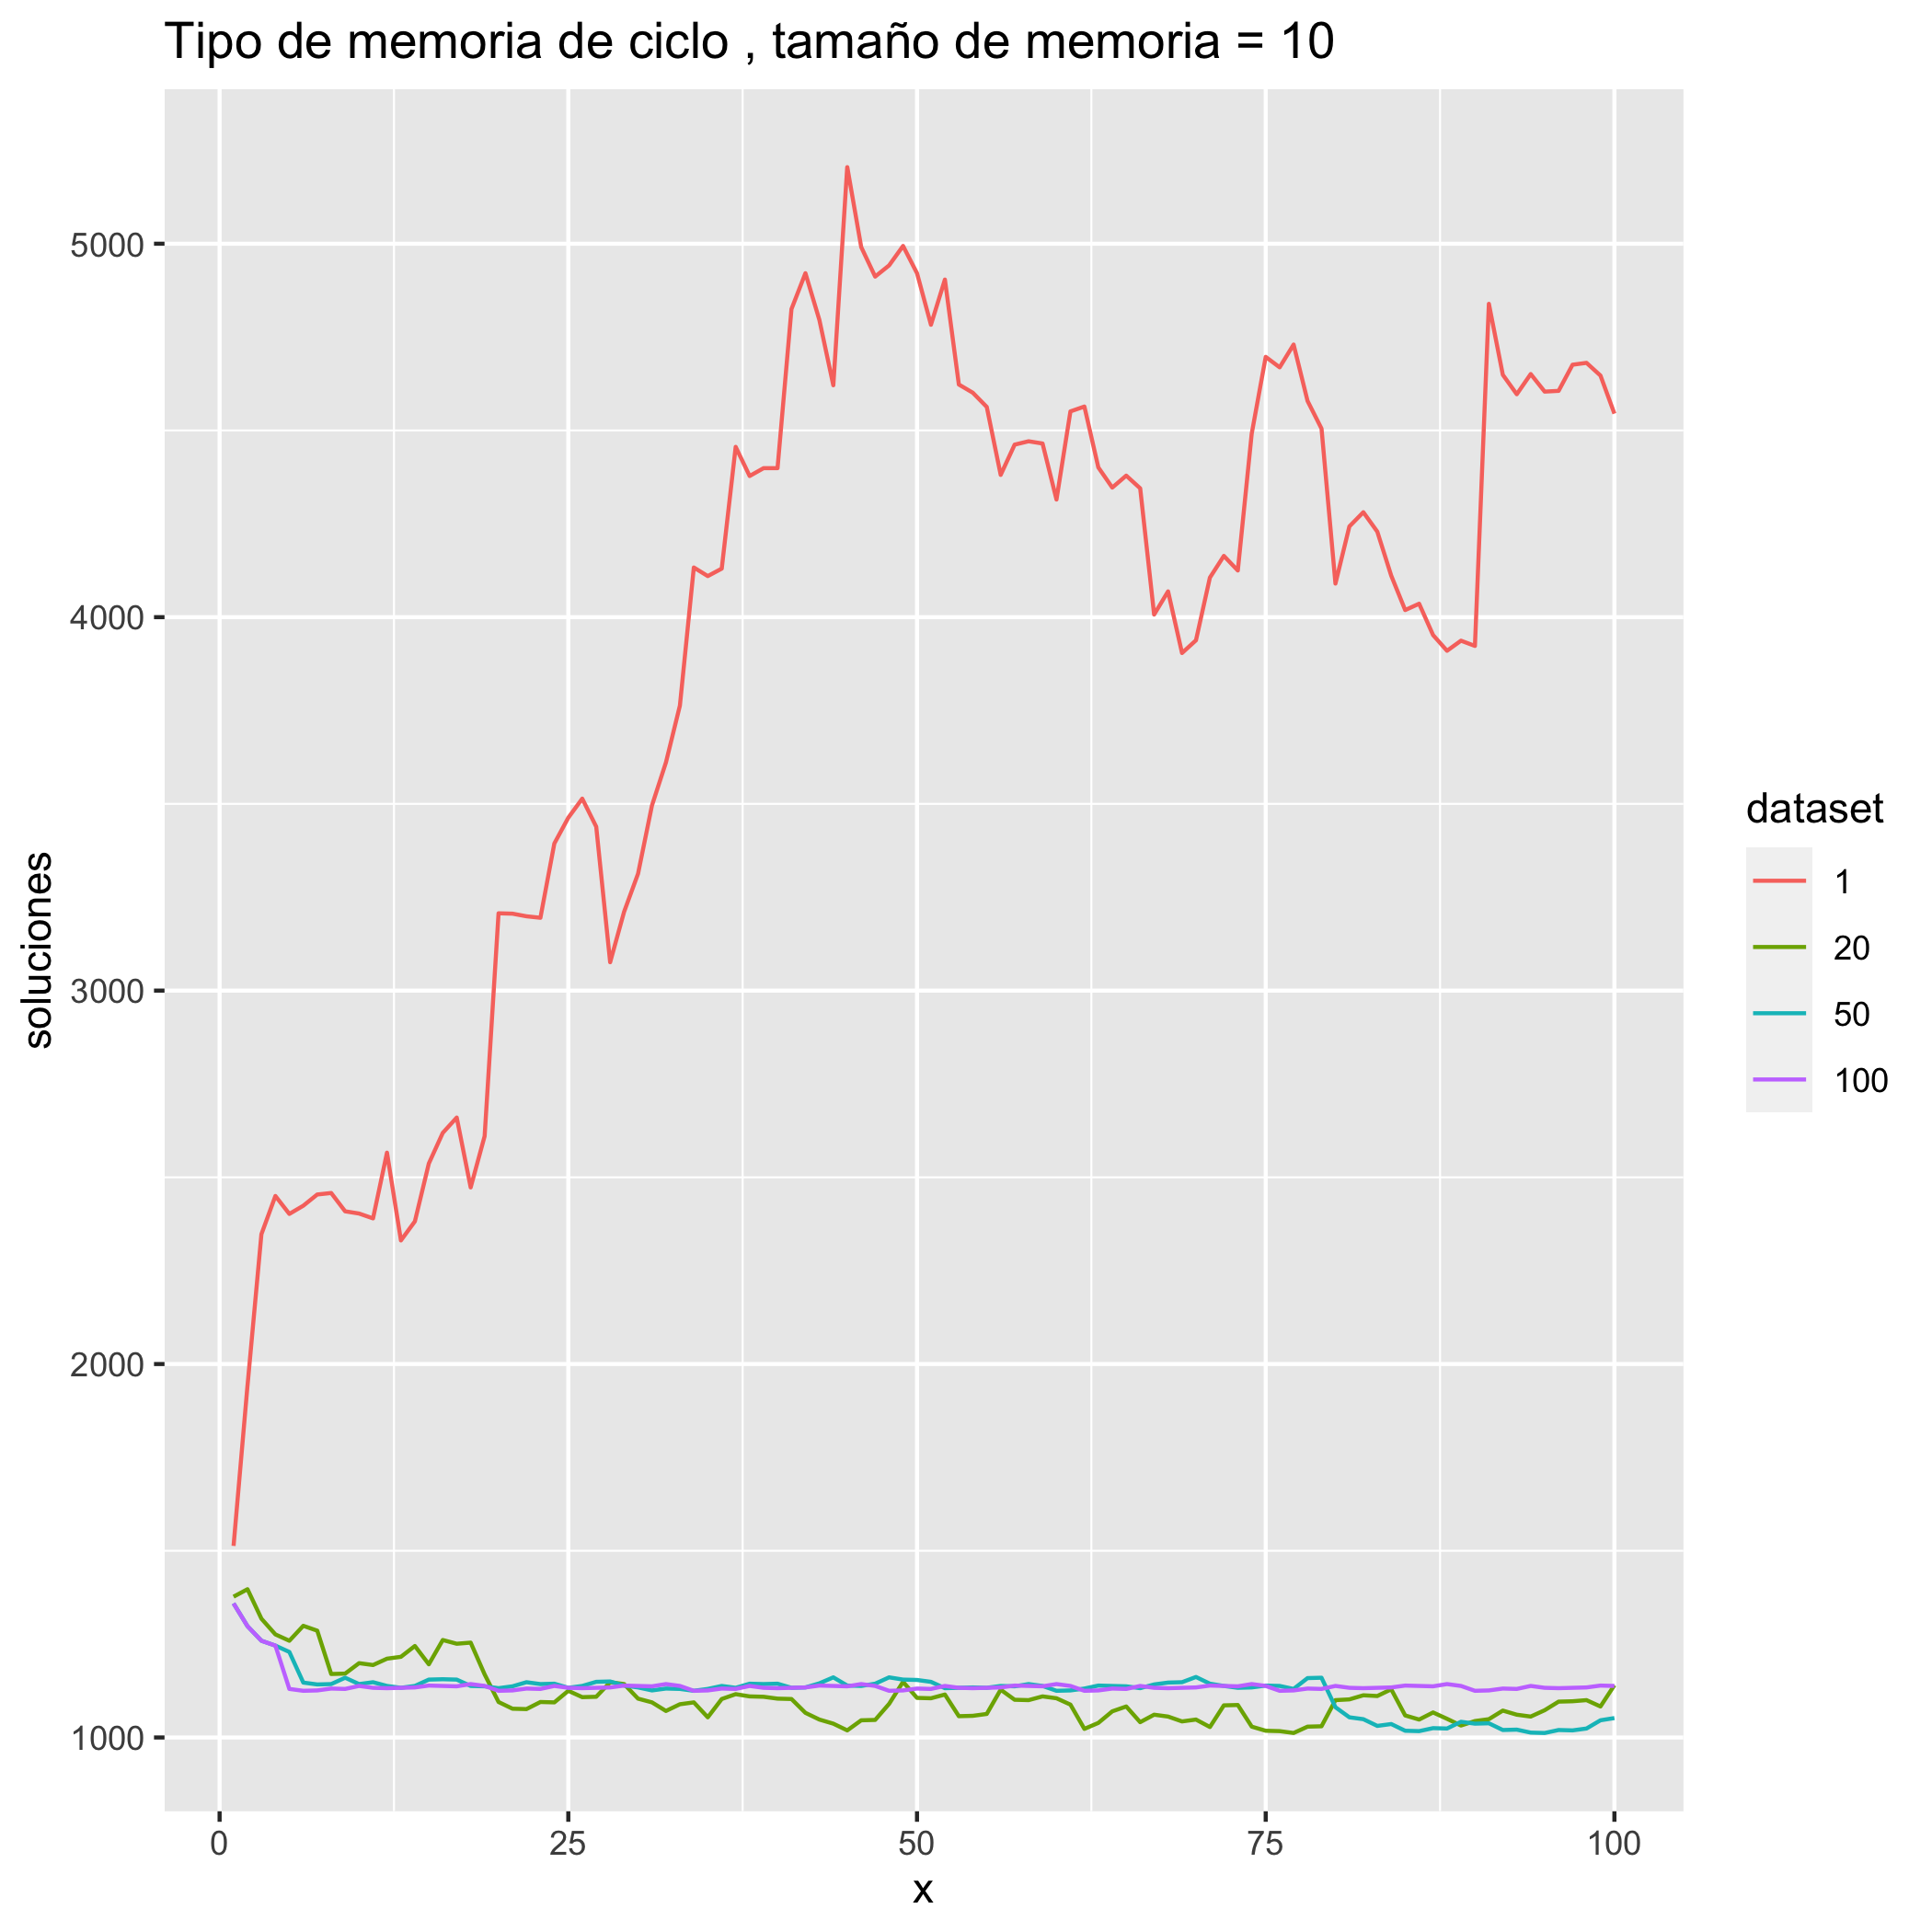
\includegraphics[scale=0.15]{img/grafico.png}
    \caption{comparación subvecindad}
    %\end{subfigure}
    \label{fig:sv}
\end{figure}

Como podemos apreciar, con subvecindad 1 el algoritmo se mueve a distintas soluciones de manera errática  entre iteraciones, devolviendo soluciones muy variadas, mientras que con mayor subvecindad las soluciones que va encontrando son más cercanas entre sí y por lo tanto es mas fácil que vaya mejorando, mientras que en el extremo de subvecindad 100 el algoritmo se comporta similar a búsqueda local, quedándose solo en soluciones muy similares, sin poder salir de su vecindario. \\

Siguiente comparamos tamaño de memoria:

\begin{figure} [H]
    \centering
    %\begin{subfigure}{0.5\linewidth}
    %\centering
    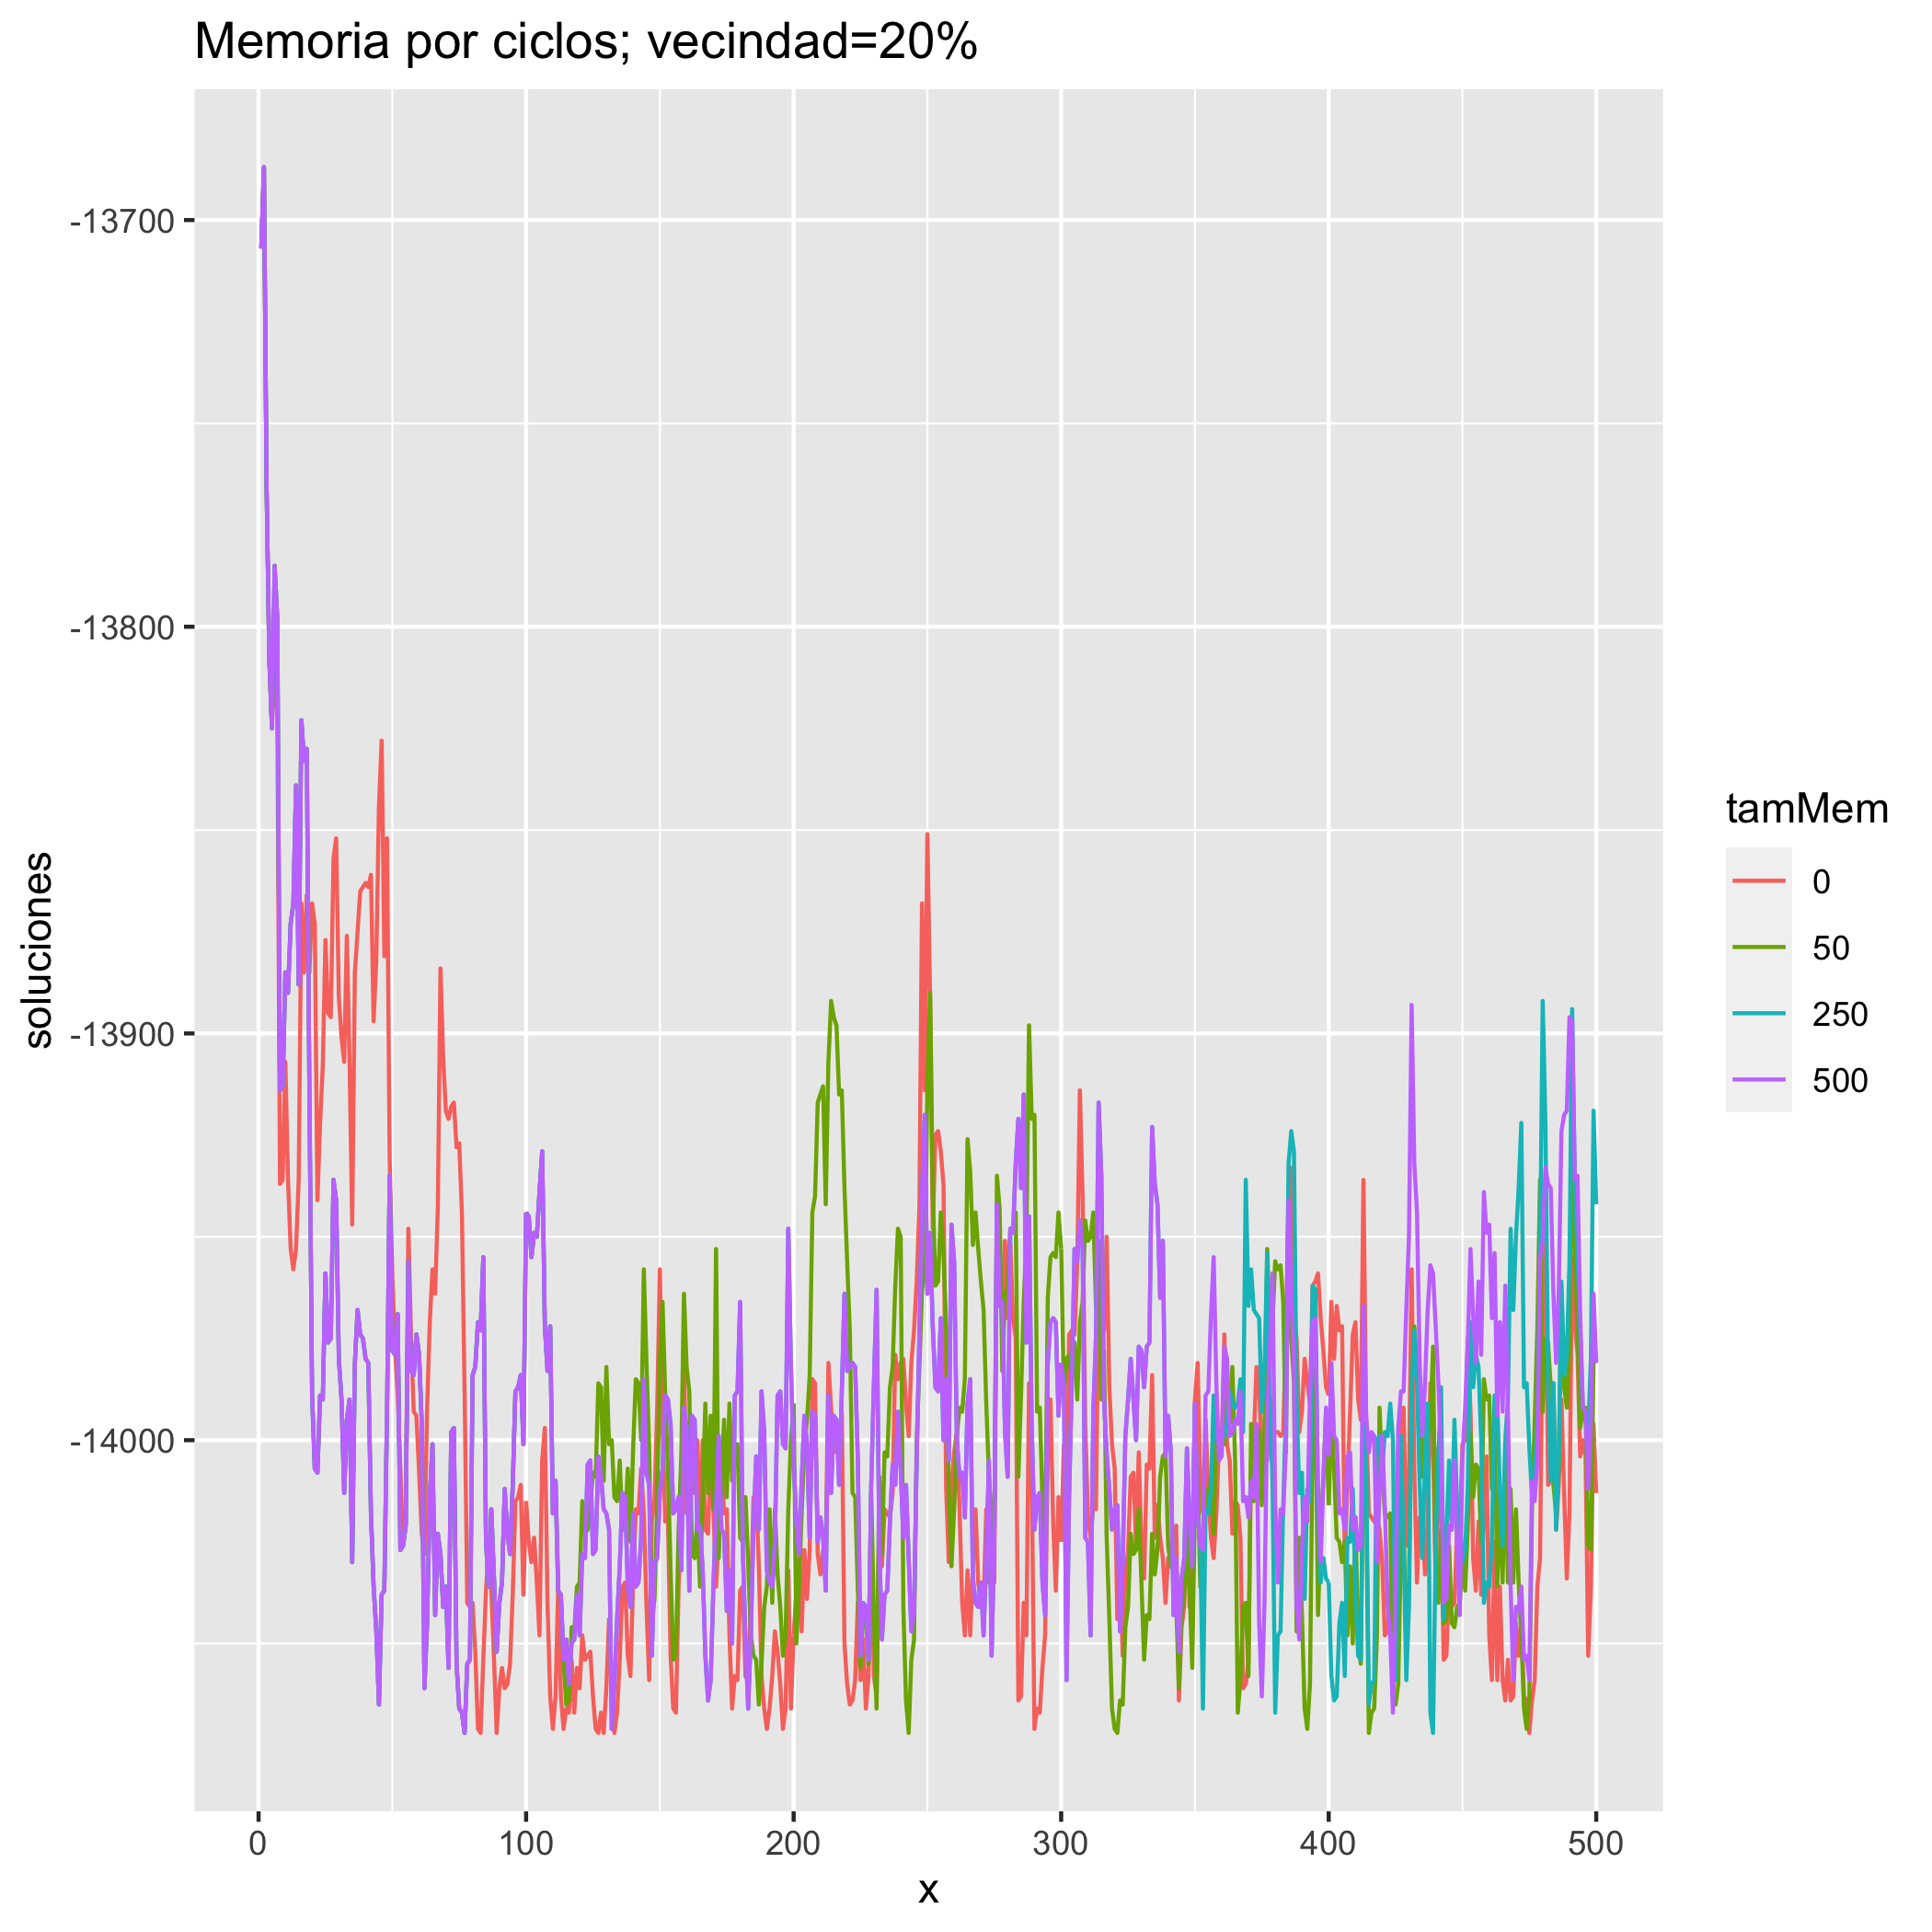
\includegraphics[scale=0.1]{img/grafico__memoria_ciclos_vecindad20.png}
    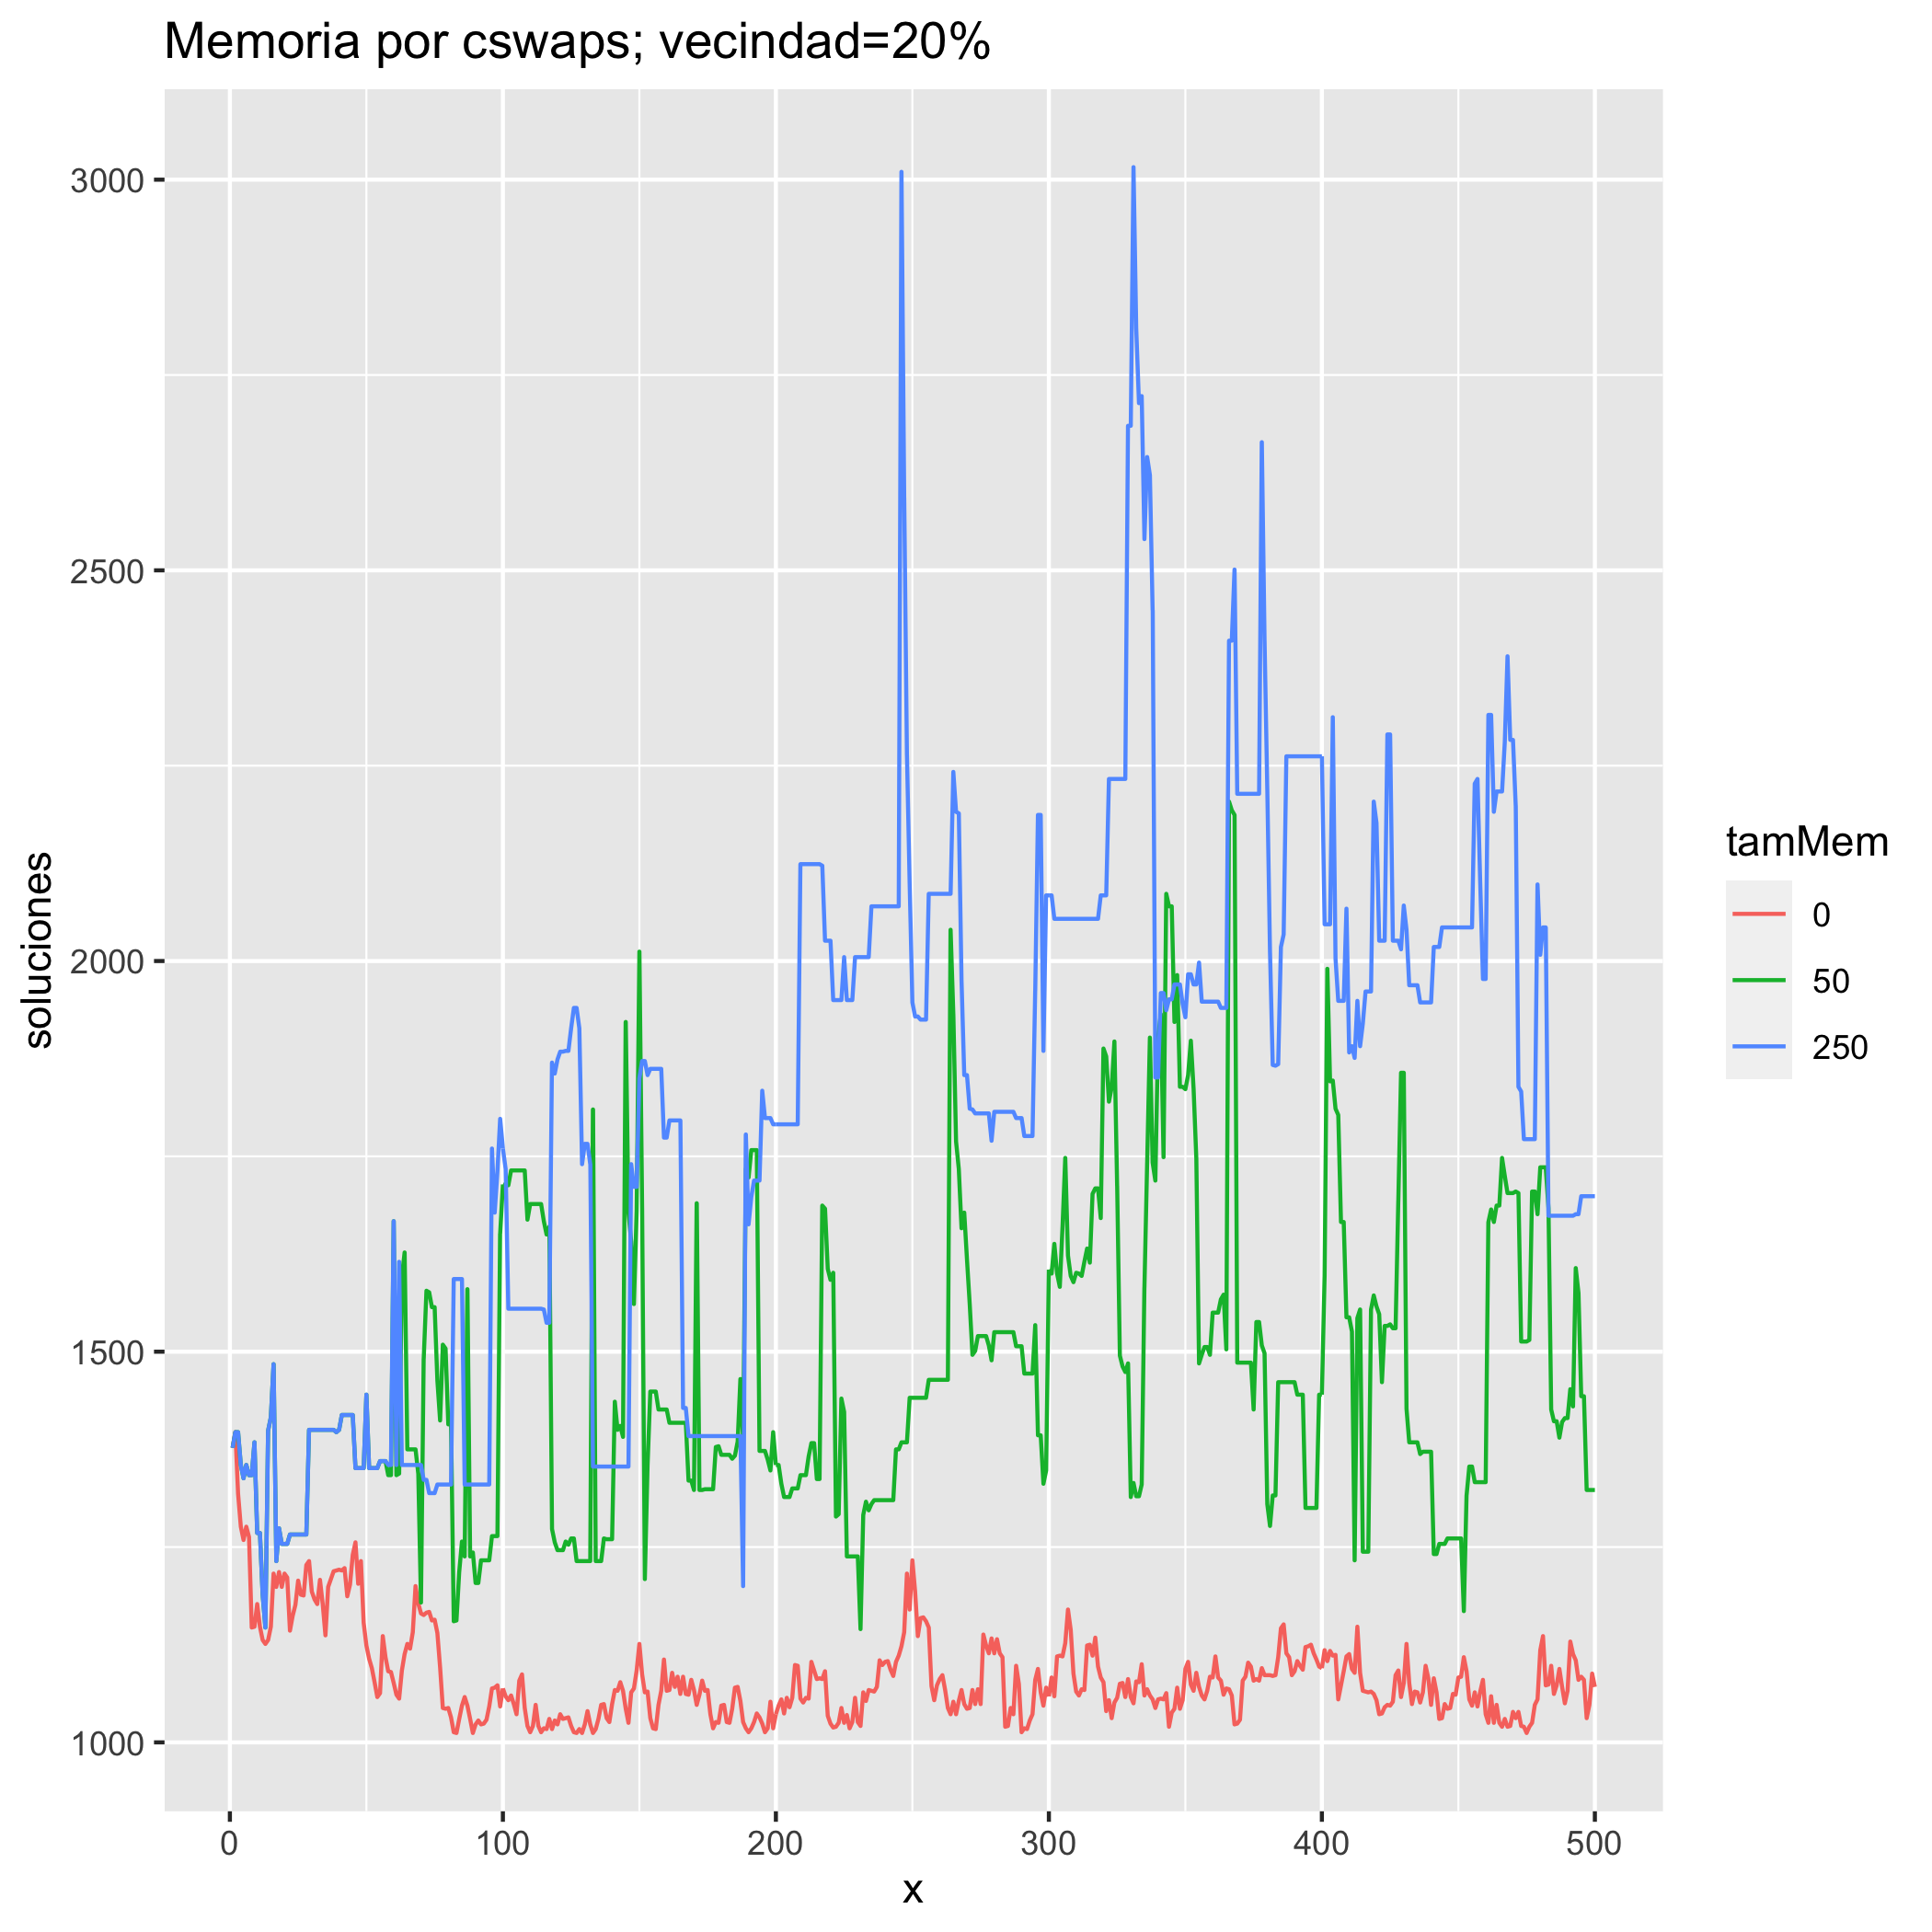
\includegraphics[scale=0.1]{img/grafico__memoria_swaps_vecindad20.png}
    \caption{comparación tamaños por tipo de memoria}
    %end{subfigure}
    \label{fig:tamMemo}
\end{figure}

En la figura \ref{fig:tamMemo} podemos observar que, cuando se trata de memoria por ciclos, el tamaño no afecta mucho a que tipo de soluciones se mueve, siendo todos los tamaños similares en cuanto a como se mueven entre soluciones por iteración. \\

Por otro lado, vemos que si la memoria almacena los $swaps$, mientras mas grande es la memoria, las iteraciones se empiezan a mover a soluciones peores ya que este tipo de memoria bloquea las soluciones posibles al bloquear movimientos en vez de ciclos.

\\
\begin{figure} [H]
    \centering
    %\begin{subfigure}{0.5\linewidth}
    %\centering
    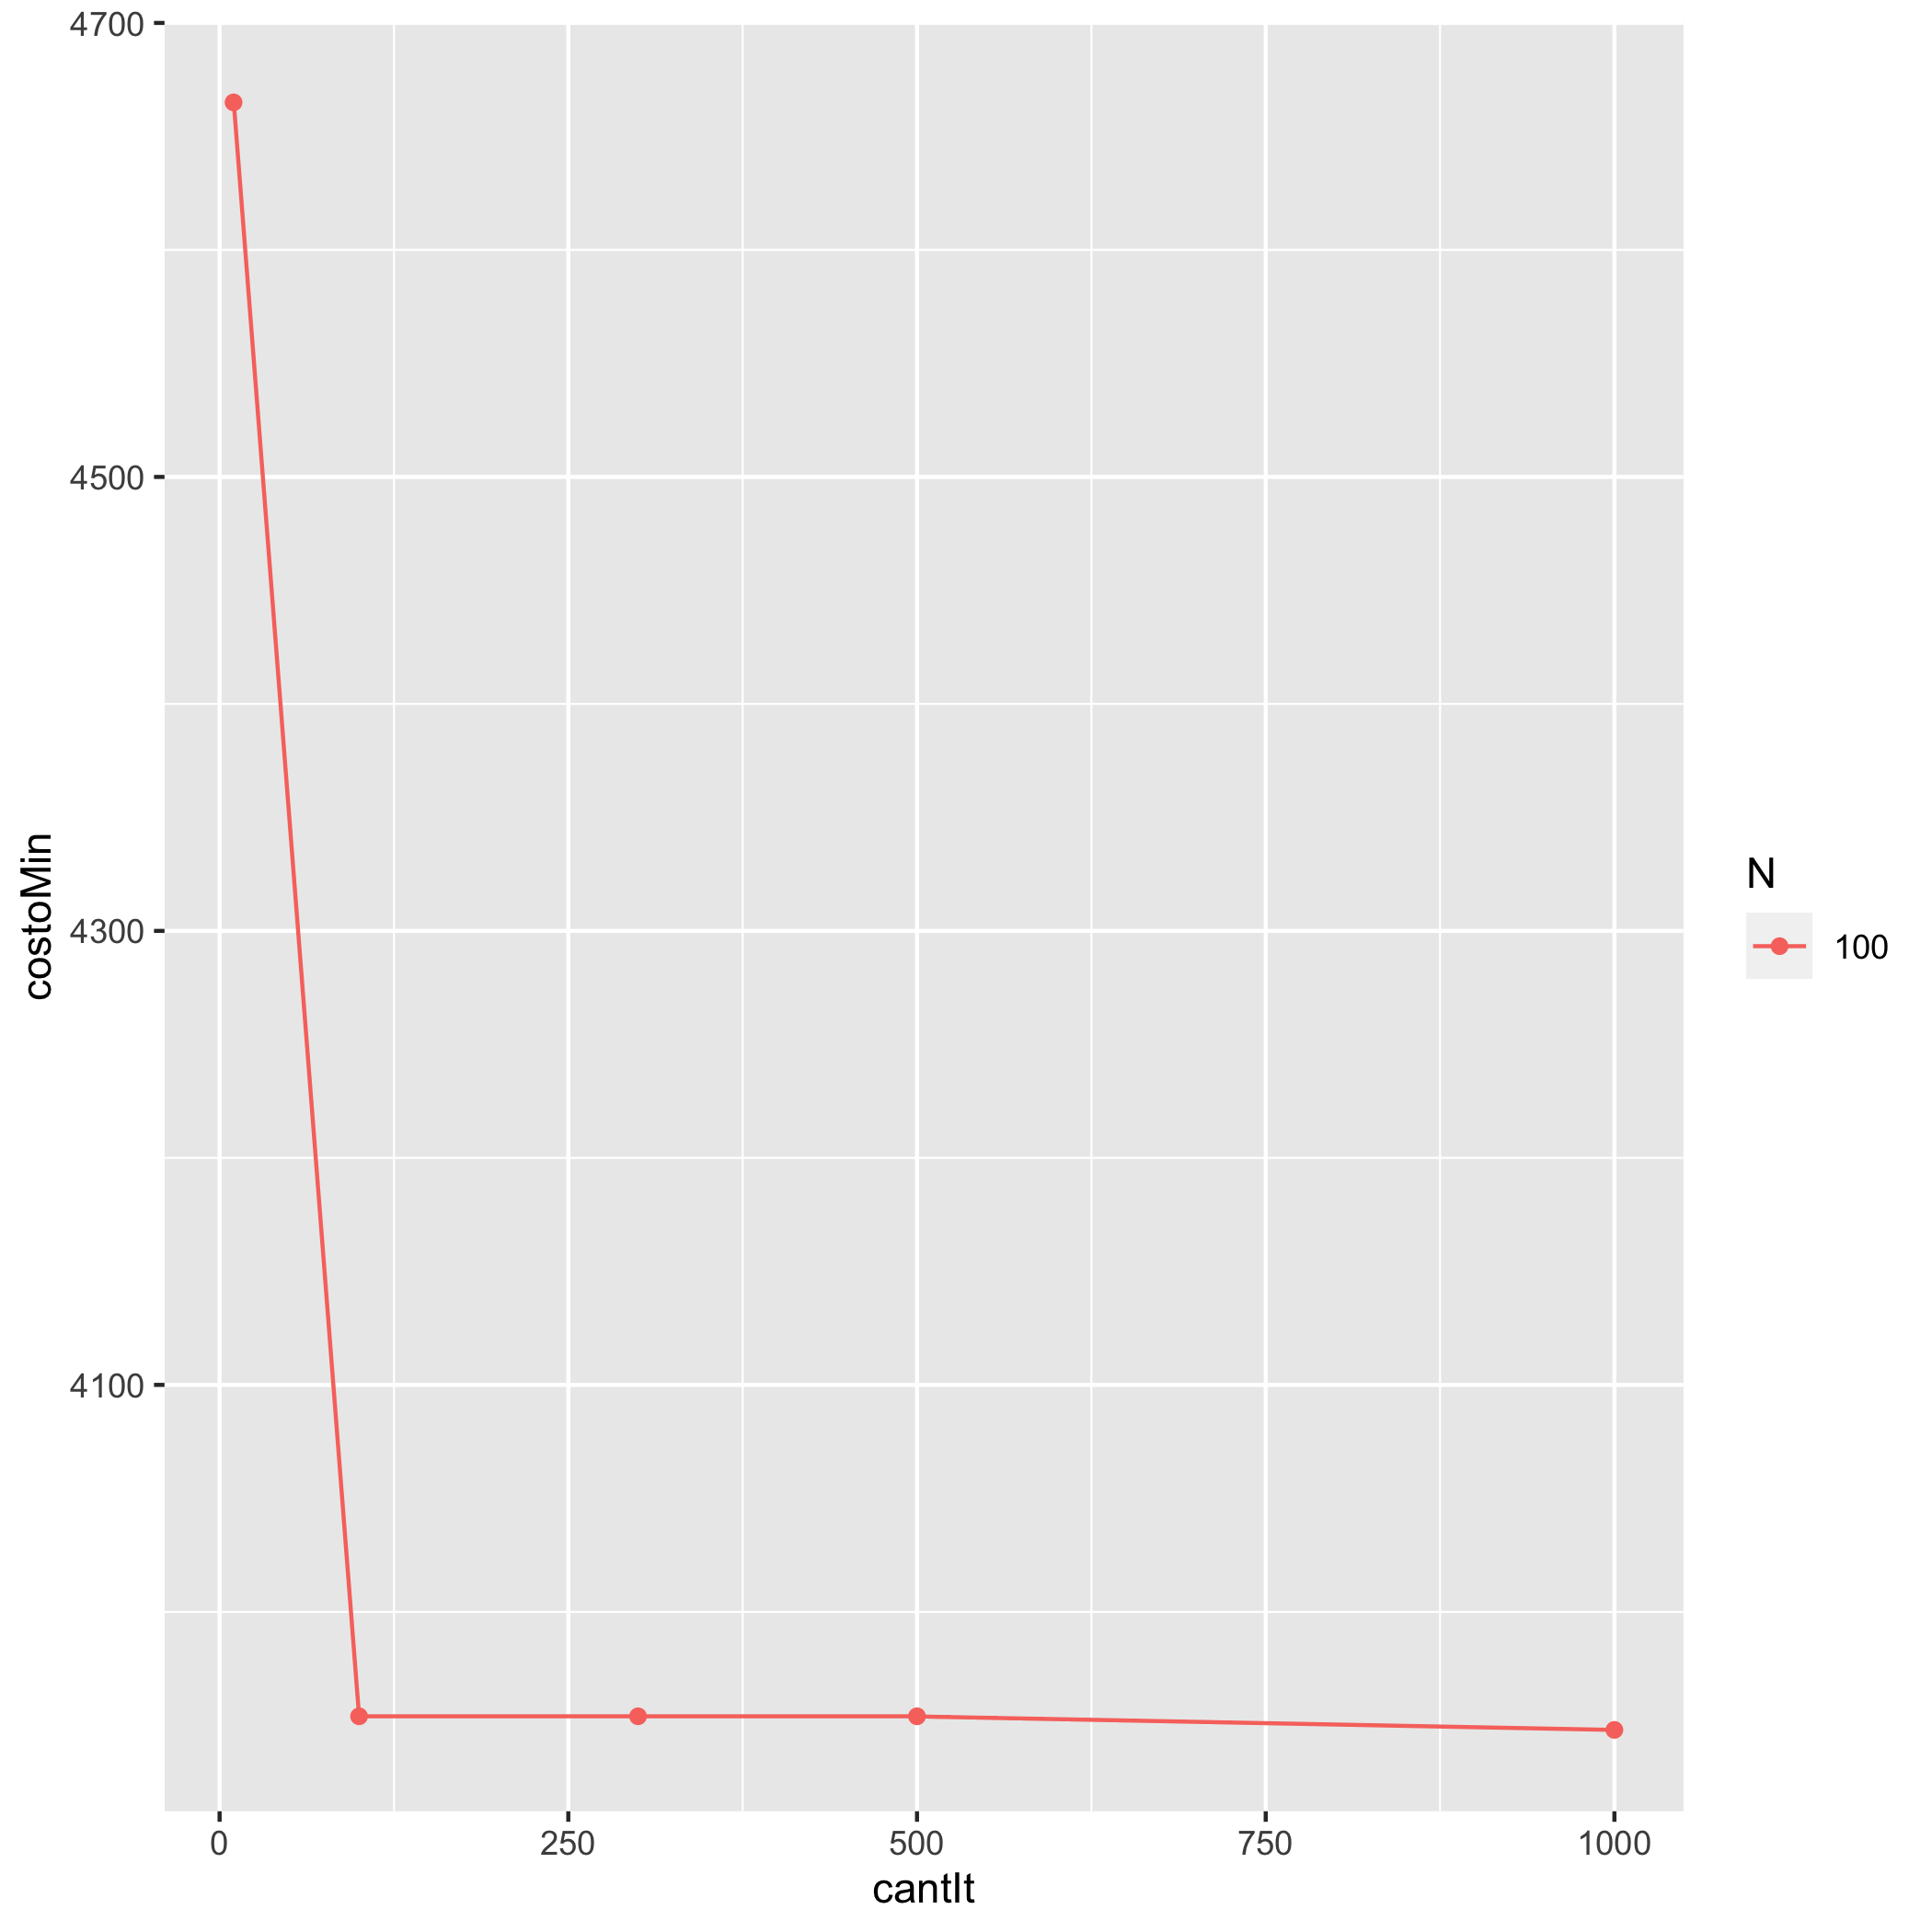
\includegraphics[scale=0.15]{img/iteracionesTabu.png}
    \caption{comparación iteraciones}
    %\end{subfigure}
    \label{fig:it}
\end{figure}

Para la cantidad de iteraciones sabemos que mientras mas hagamos, más posibilidades de encontrar una solución mejor, por lo tanto hacer más iteraciones es mejor con respecto a sacar un mejor óptimo, pero afecta de gran manera al tiempo de ejecución final.

%y alguna que otra cosa que veamos de los graficos
\\
Con los resultados obtenidos en nuestro análisis, concluimos que mientras mayor cantidad de iteraciones la solución va a ser mejor, también vemos que el tipo de memoria por ciclos es mas consistente para encontrar nuevas y mejores soluciones sin importar mucho su tamaño, y una subvecindad medianamente baja es mejor para poder recorrer mayor cantidad de vecinos distintos, sin llegar a comportarse de manera errática viendo soluciones muy alejadas de la óptima.

\subsection{experimentos con datasets propios}
Para estos experimentos vamos a utilizar los siguientes datasets:
\begin{itemize}
\setlength{\itemsep}{1pt}
\setlength{\parskip}{0pt}
 \setlength{\parsep}{0pt}
    
\item \textbf{random}:instancias con N que va de 10 a 50 donde las aristas tienen pesos similares.
\item \textbf{randomVariacionAlta}:instancias con N que va de 10 a 50 donde las aristas tienen una variación grande de peso entre sí.

\end{itemize}

Con las consideraciones anteriores sobre los parámetros a usar en tabú, vamos a comparar los cuatro algoritmos pedidos, en cuanto a tiempo y calidad de resultado final. Para tabu vamos a utilizar cantIteraciones 1000, memoria de 300, subvecindad de $20$ en los dos tipos de memoria
\\
%Aca la idea serian comparaciones de los 4 algos, tomando en cuenta tanto tiempo como cual es una solución de costo menor.
\begin{figure} [H]
    \centering
    %\begin{subfigure}{0.5\linewidth}
    %\centering
    \includegraphics[scale=0.15]{img/tiempos.png}
    \caption{comparación tiempos por algoritmo}
    %\end{subfigure}
    \label{fig:tiempos}
\end{figure}

Primero aclaramos que TABU:0 representa tabú por memoria de ciclos mientras que TABU:1 representa memoria por swaps.
Con eso en cuenta, vemos que en la figura \ref{fig:tiempos} podemos diferenciar claramente que cada algoritmo tiene tiempos distintos menos BG y AGM que tienen tiempos similares.
A su vez podemos ver que tabú cuando es memoria por swaps es mas rápida que por ciclos como explicamos en la parte de complejidad del algoritmo \ref{alg:TABU}.
\\
%posiblemente decir algo con respecto a que tabu tarda considerablemente mas pero da mejores soluciones.
\begin{figure} [H]
    \centering
    %\begin{subfigure}{0.5\linewidth}
    %\centering
    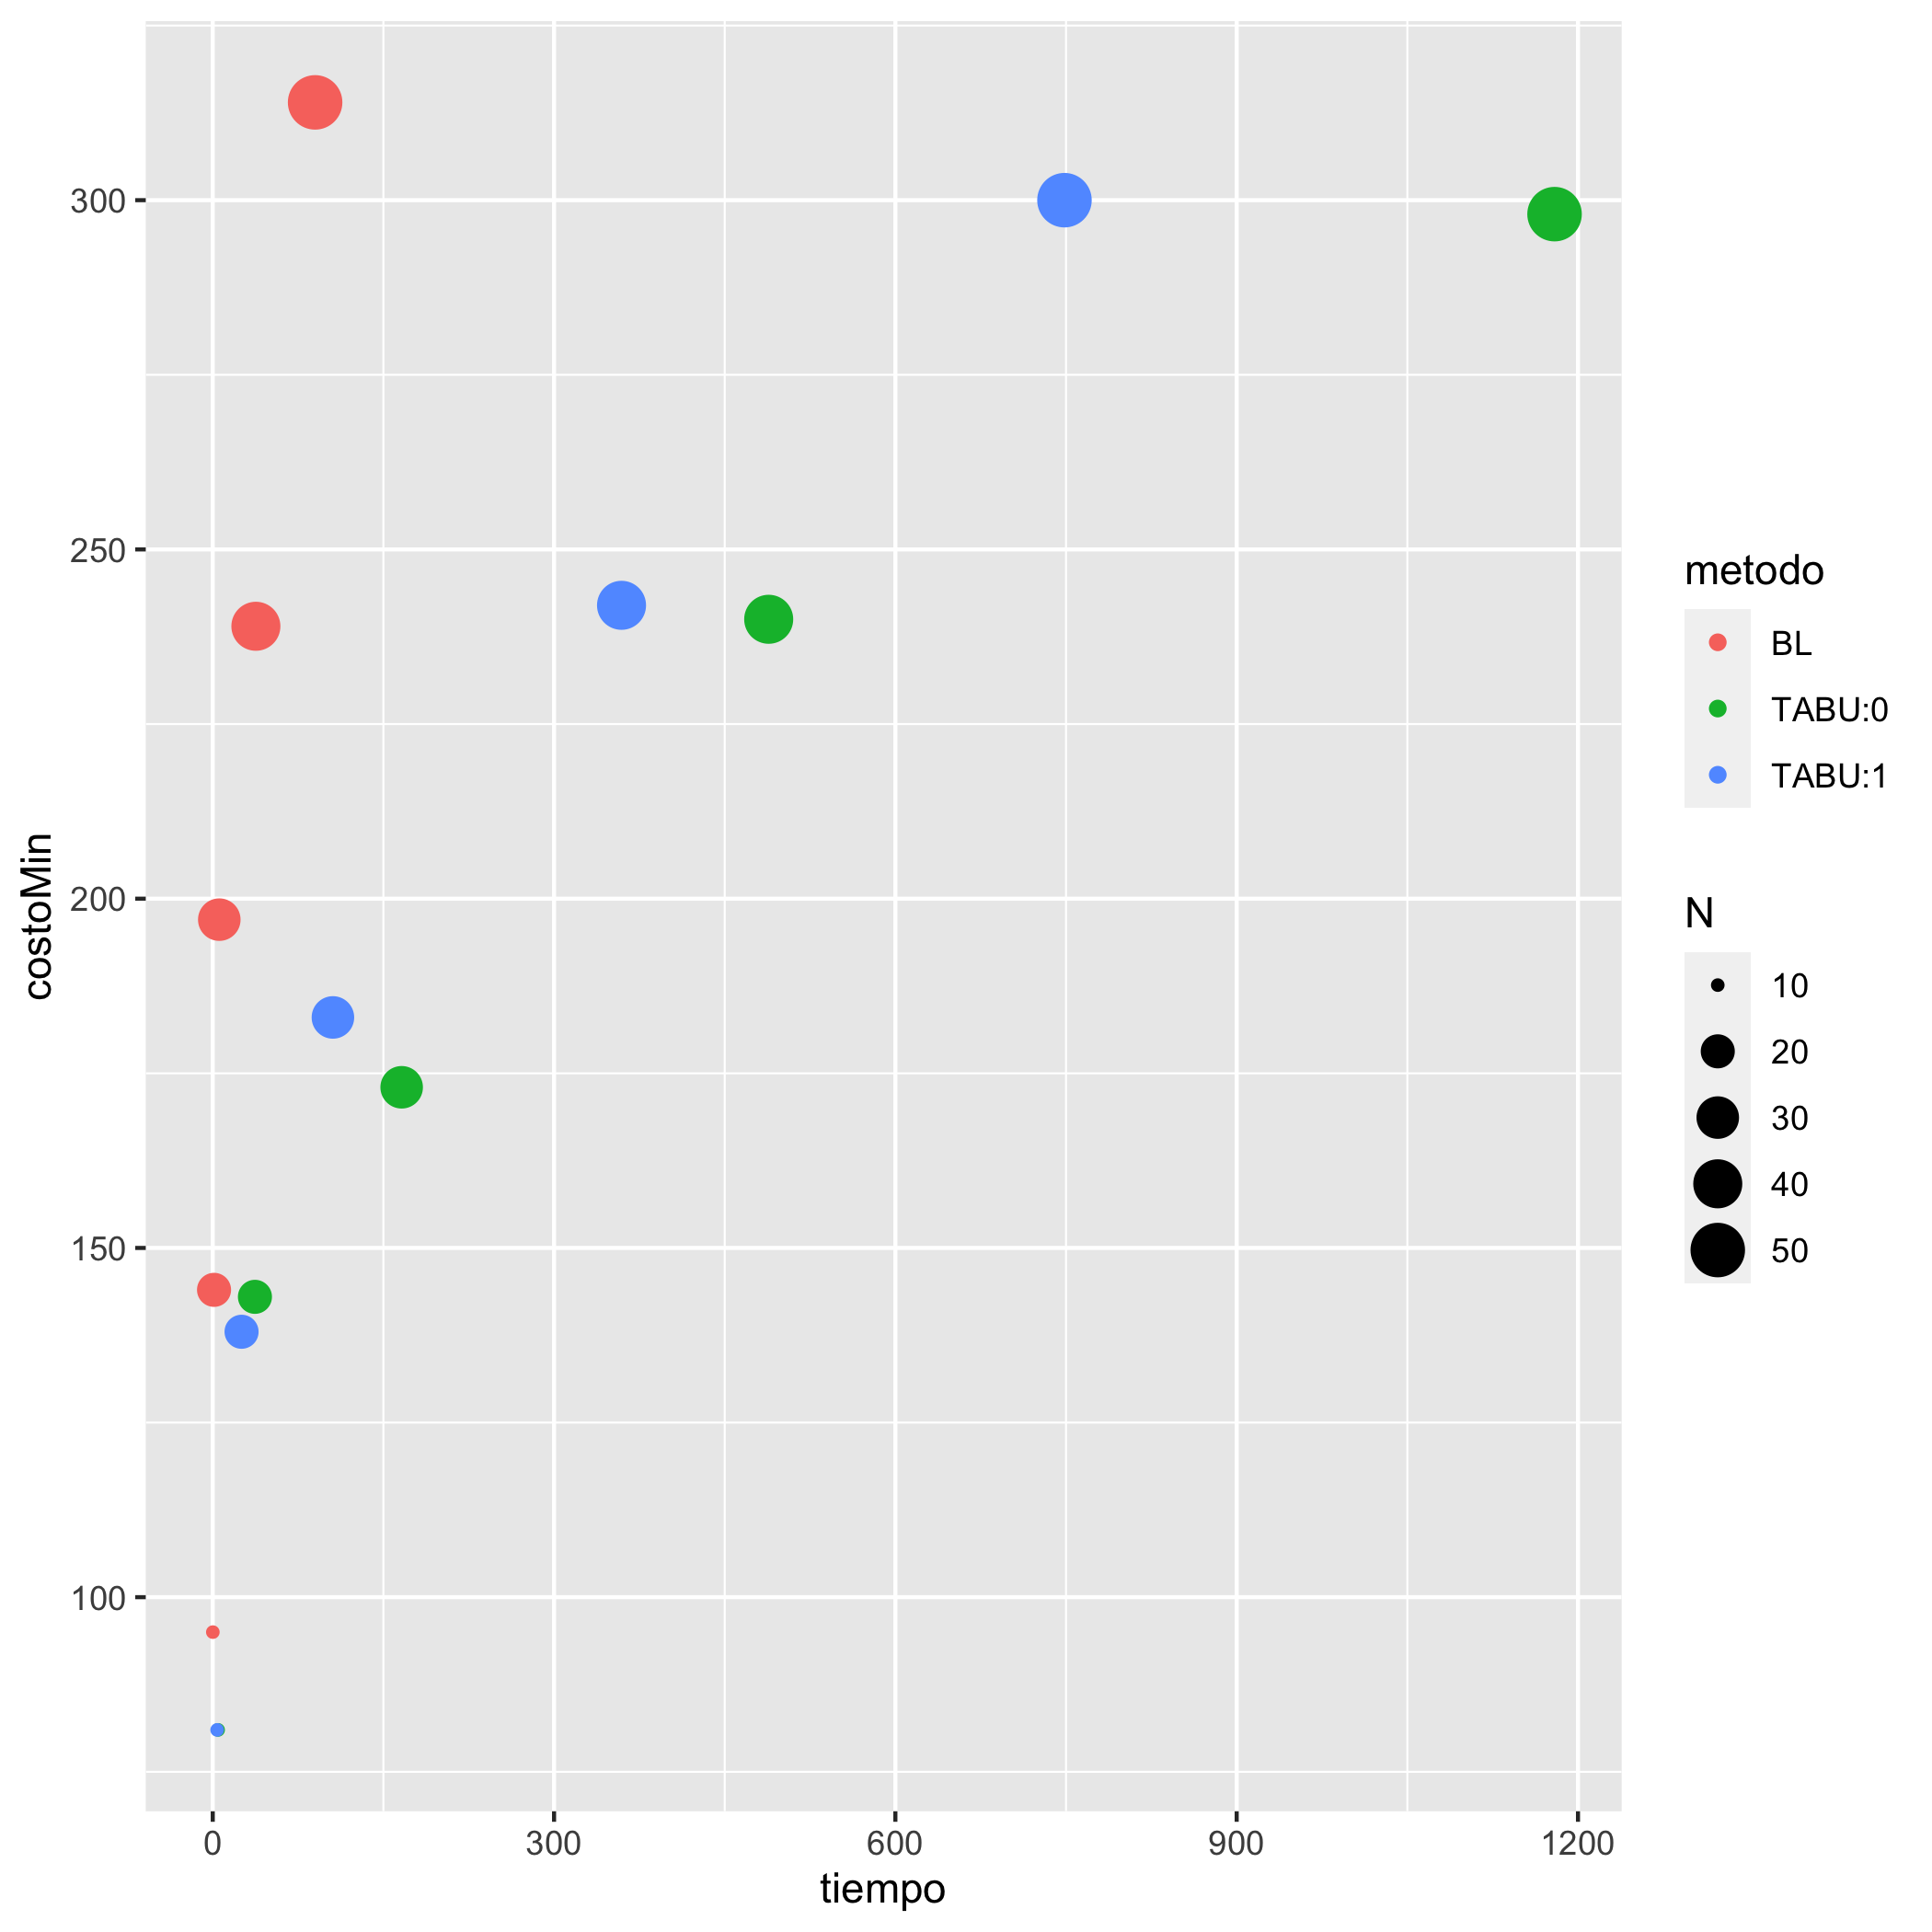
\includegraphics[scale=0.15]{img/CalidadvsTiempo.png}
    \caption{comparación calidad solución entre tabu y local}
    %\end{subfigure}
    \label{fig:calidad}
\end{figure}
%y alguna que otra cosa que veamos de los graficos

En la figura \ref{fig:calidad} se puede observar la comparación entre tiempo y solución óptima hallada. Podemos notar que tabú es considerablemente más lento que búsqueda local, pero devuelve mejores soluciones en la mayoría de casos. Por otro lado, apreciamos que la búsqueda local devuelve un resultado bastante cercano a la que brinda tabú en un tiempo mucho menor.\\
Por lo tanto podemos concluir que en casos donde N sea muy grande, si se necesita obtener una solución rápida, realizar búsqueda local va a brindar una respuesta aceptable en poco tiempo, mientras que si se dispone de mucho tiempo, no hay razón para no utilizar tabú y obtener un mejor resultado.

\section{Conclusión}

Para el desarrollo de este trabajo, como bien se explicó y presentó a lo largo de este trabajo, se utilizaron cuatro algoritmos, algunos distintos entre si y otros basados en el anterior, inclusive alguno mejorado otro.

Para empezar, los algoritmos mas sencillos como la búsqueda golosa o la heurística basada en AGM son aquellos que, en tiempo de ejecución, son rápidos para brindar una respuesta no obstante, la misma puede no ser la óptima incluso con un ratio de error bastante grande, pero para obtener un resultado y poder operar, son bastante eficaces.

Entre estos dos algoritmos, su comparación de resultados, podemos decir que la Búsqueda Golosa nos brindó resultados mucho mas cercanos a los óptimos que se han encontrado al momento para varios ejemplos tales como Berlin52, ST70, Ulysses16, Kroe100.

Por otro lado, tenemos el algoritmo de Búsqueda Local que dada una de las dos soluciones previas de goloso y AGM se enfoca en encontrar una mejor a partir de ciertos cambios en el camino. Este algoritmo en relación de tiempo puede ser un poco peor que los anteriores, pero para encontrar un mejor resultado, es mucho mejor a la hora de dar soluciones mucho mas cercanas al óptimo. En relación al tiempo de ejecución con los dos algoritmos previos, este es el que más tiempo demora en ejecutarse para dar una solución.

Para finalizar, tenemos al algoritmo basado en la búsqueda tabú que, en términos generales, fue aquel que mejores resultados nos ha brindado dándonos soluciones más cercana a los óptimos encontrados hasta el momento en diversos ejemplos. No obstante, el uso de las componentes que se explicaron en su sección, ocasiona que el algoritmo pueda extender su tiempo de ejecución en una muy pero muy amplia diferencia y también pueda ocupar mas recursos de la computadora tal como la memoria ya que, para extender mejores soluciones, almacena caminos enteros y, para grafos con muchos nodos, esta diferencia puede crecer bastante.
Si lo comparamos con los tres algoritmos previos, este es el que más recursos y tiempo consume no obstante, es el que mejor resultados brinda en todos los casos

Entre todos estos algoritmos, si se necesita una respuesta rápida y efectiva, podemos usar la Búsqueda Local para tener una mejor respuesta, sin embargo, si necesitamos una solución mas cercana al óptimo, la búsqueda local resulta darnos mejores resultados

Teniendo estas conclusiones previas sobre cada algoritmo, una futura actividad a tener presente para una posible mejora, es probar en la heurística del AGM otro algoritmo de generación de Árbol tal así como Kruskal. Proponemos este cambio ya que, contrario al algoritmo de Prim que va generando un árbol a lo largo del grafo, Kruskal genera bosques y, la elección de como arma esos bosques, puede afectar al resultado final dando otros resultados y podría ser un buen punto de partida comparar los resultados obtenidos.

También otro objetivo puede ser, probar con otras estructuras de representación de grafos tales como Matriz de Adyacencia o Lista de Adyacencias de forma que para comparar tiempo de ejecución ya que alguna estructura puede obtener datos como aristas o valores en tiempo O(1) y esto puede reducir las ejecuciones considerablemente.

\end{document}
